\begin{figure}[tbp] 
  \centering
  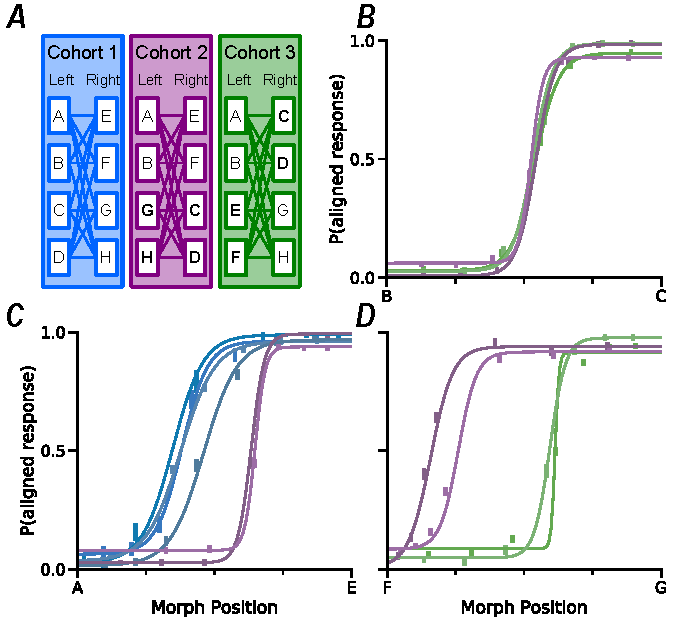
\includegraphics[width=114mm]{figures/fig03_shift.pdf}
  \caption[Different training context sometimes results in reliable shifts in the psychometric curves]
{
(A)	Diagram of alternative training contexts. Task structure remains the same in each cohort, but some motif category assignments change. Category assignment differences from Cohort 1 are bolded in Cohort 2 and 3. This allows a subset of the morph dimensions to be compared across training on different category permutations. Colors correspond to colors used in adjacent plots.
(B-D)	Exemplar psychometric curves from subjects trained on different category permutations. 
(B)	On most dimensions the boundary is conserved as if the training was the same as shown in the psychometric curves from these 4 birds, 2 from each of cohort 2 (purple) and cohort 3 (green) along the morph dimension between motif B and motif C. 
(C-D)	However, on some of the dimensions, such as A to E (left) and F to G (right), the behaviorally measured boundaries depend on the initial categorical assignment.  When there is a difference, the boundaries are still conserved within cohorts.
\index{shift}}
  \label{fig:shift}
\end{figure}